\documentclass[../../../main.tex]{subfiles}

\begin{document}
    Schließlich untersuchen wir noch das Verhältnis der Pumpleistung $P_p$ und Laserleistung $P_a$. Abbildung zeigt die experimentellen Daten.

    \begin{figure}[H]
        \centering
        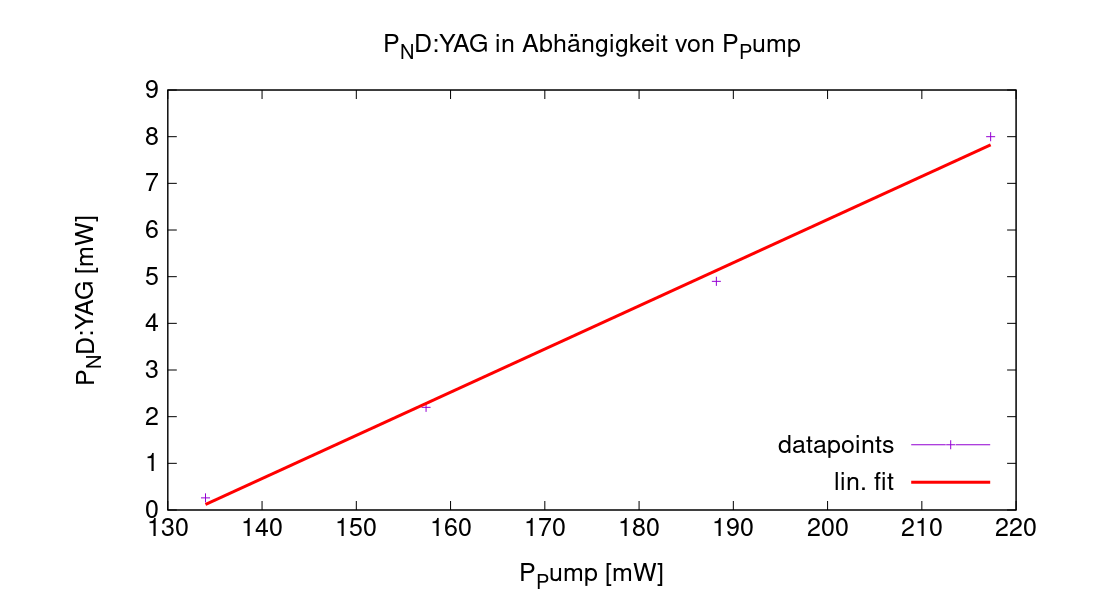
\includegraphics[width=11cm]{../../Bilddateien/5/P(NDYAG)overP(Pump).png}
        \caption{Die Laserleistung $P_a$ als Funktion der Pumpleistung $P_p$}
        \label{fig:PumpLaserLeistung}
    \end{figure}

    Gleichung \eqref{eq:Grundlagen:Pumpleistung} aus der Theorie sagt einen linearen Zusammenhang voraus, weswegen ein Fit folgener Form angelegt wurde:
    \[
        f_{a,b}(x) := a\cdot (x - b).      
    \]
    Die relevanten Parameter des Fits sind in Tabelle \ref{tab:PumpLaserLeistungFitParameter} zu sehen.

    \begin{table}[H]
        \centering
        \begin{tabular}{c|cc |cc}
            \hline
            & $a$ in $\si{\per\milli\W}$ & $u(a)$ in $\si{\per\milli\W}$ & $b$ in $\si{\milli\W}$ & $u(b)$ in $\si{\milli\W}$\\
            \hline\hline
            $f_{a, b}$ & 0.0925 & 0.0038 & 132.7 & 2.2
        \end{tabular}
        \caption{Die Parameter der linearen Kurvenanpassung.}
        \label{tab:PumpLaserLeistungFitParameter}
    \end{table}

    $b$ ist nach Definition des Fits gerade die Schwellleistung $P_{th}$, ab welcher der Laser Licht produziert. $a$ ist der sogenannte differentielle Wirkungsgrad $\alpha_S$. Eine genaue Inspektion von Gleichung \eqref{eq:Grundlagen:Pumpleistung},
    \[
        P_a = \underbrace{\eta\cdot\frac{E_{32}}{E_{41}}\cdot \frac{T}{T + L}}_{=\alpha_S}\cdot(P_p - \underbrace{P_{th}}_{=b}),
    \]
    erlaubt weiter die Bestimmung der Quantenausbeute $\eta$. Dabei ist $E_{32} \propto \SI{1064}{\n\m}$ die Energiedifferenz der Laserzustände, $E_{41} \propto \SI{808}{\n\m}$ die Energiedifferenz der Pumpzustände, $T=\SI{20}{\percent}$ die Transmissivität des Resonatorspiegels und $L$ die sonstige Photonen-Verlustrate. Es sei der verlustfreie Fall angenommen ($L=0$), also 
    \[
        P_a = \eta\cdot\frac{E_{32}}{E_{41}}\cdot(P_p - P_{th}) \implies \eta = \frac{E_{41}}{E_{32}}\cdot \frac{P_a}{P_p - P_{th}}.
    \] 
    Einsetzen aller $P_a, P_p$-Messwerte liefert je einen Wert von $\eta$, mit fortgepflanzter Unsicherheit. Im Mittel ergibt sich dann $\eta = \SI{9.01(77)}{\percent}$ mit kombinierter Unsicherheit der Einzeleregebnisse\footnote{Die Unsicherheit der Quantenausbeute für eine Pumpleistung von $\SI{134}{\milli\w}$ wurde bei Bildung der Unsicherheit des Mittelswerts vernachlässigt. Grund hierfür ist, dass die Pumpleistung recht nahe bei der Schwellleistung liegt, also $1/ (P_p - P_{th})$ groß wird und selbst bei kleinen Abweichung der zugehörigen Laserleistung vom Fit zu unrealistisch großen Unsicherheiten führt}. Um das Ergebnis in den realen Fall nichtverlustfreier Resonatoren ($L\neq 0$) einordnen zu können, wird noch die Quantenausbeute $\eta$ über die Resonatorverluste aufgetragen:
    \[
        \alpha_S = \eta(L)\cdot\frac{E_{32}}{E_{41}}\cdot\frac{T}{T + L}\implies \eta(L) = \alpha_S\cdot\frac{E_{41}}{E_{32}}\cdot\frac{T + L}{T}.
    \]
    Das Ergebnis ist in Graph \ref{fig:Auswertung:5:VerlustAusbeute} gezeigt.

    \begin{figure}[H]
        \centering
        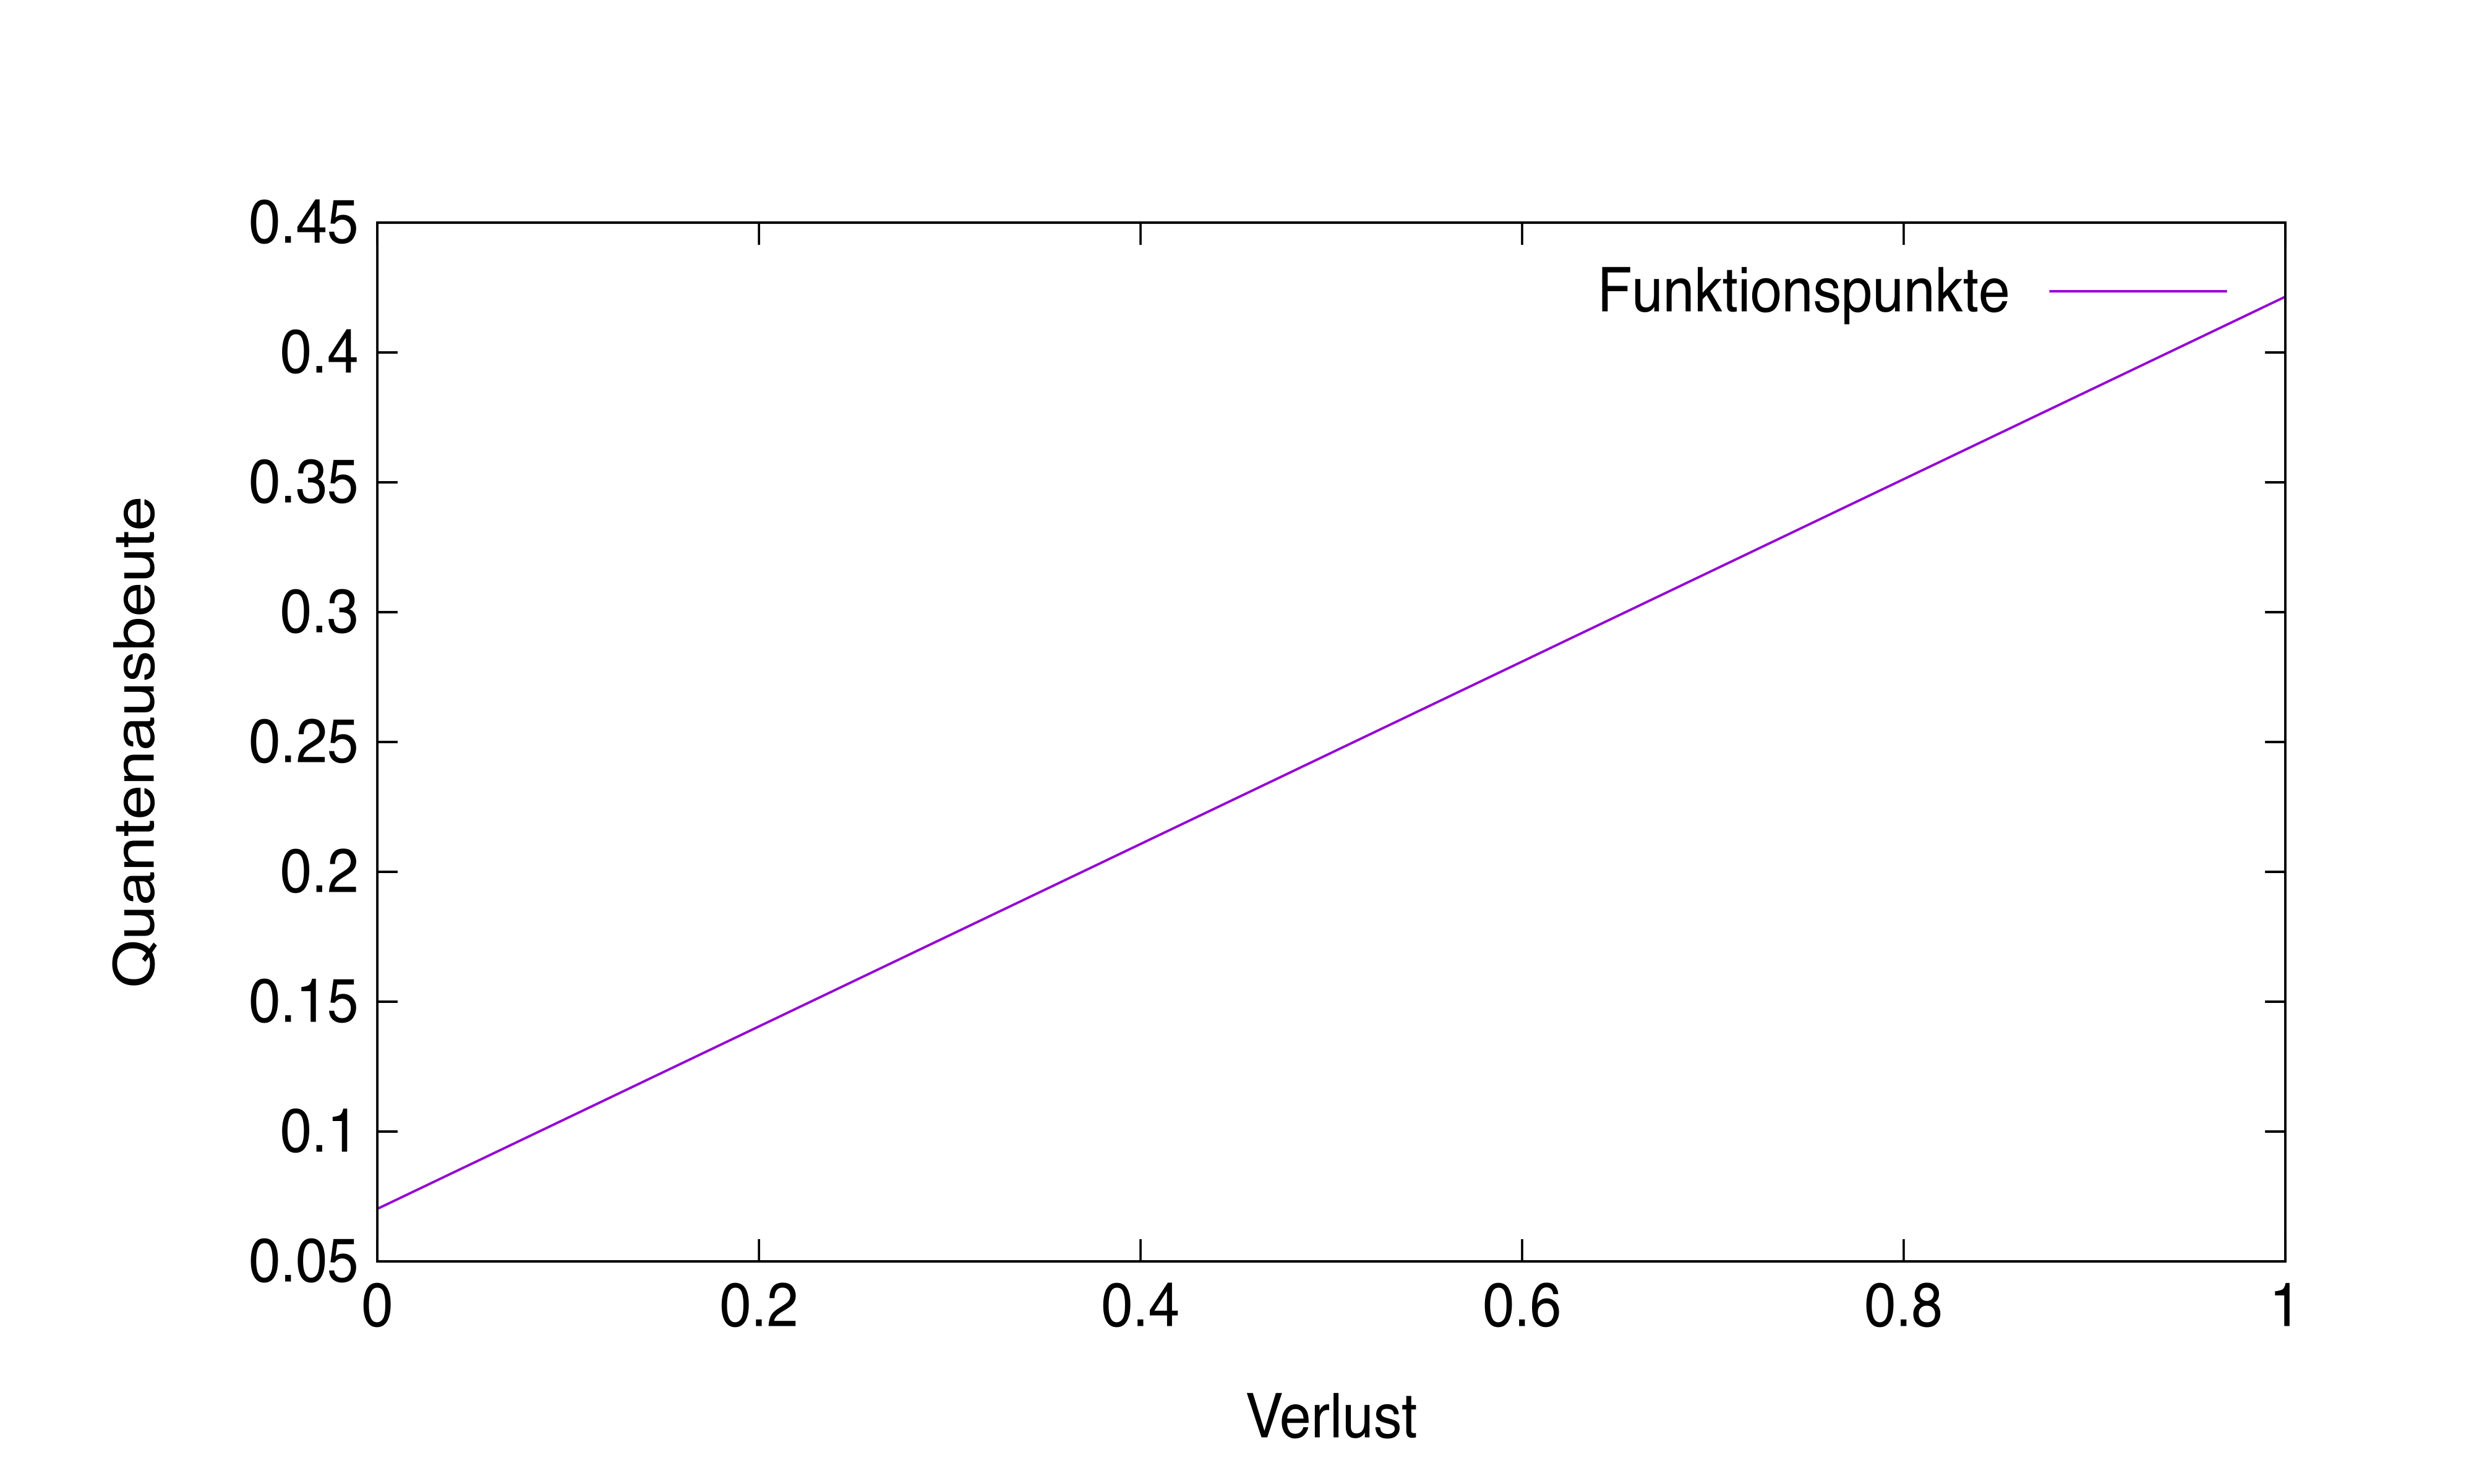
\includegraphics[width=11cm]{../../Bilddateien/5-1/VerlustAusbeute.png}
        \caption{Die Quantenausbeute bei gemessenen Wirkungsgrad $\alpha_S$ aufgetragen über die Photonenverlustrate $L$ im Resonato}
        \label{fig:Auswertung:5:VerlustAusbeute}
    \end{figure}



\end{document}